%%%%%%%%%%%%%%%%%%%%%%%%%%%%%%%%%%%%%%%%%%%%%%%%%%%%%%%%%%%
%\vspace{-20pt}
%\vspace{\sectionReduceTop}
\section{Introduction}
%\vspace{\sectionReduceBot}
\label{sec:intro}
%%%%%%%%%%%%%%%%%%%%%%%%%%%%%%%%%%%%%%%%%%%%%%%%%%%%%%%%%%%


We are witnessing a renewed excitement in multi-discipline Artificial Intelligence (AI) research problems. In particular, research in image and video captioning that combines Computer Vision (CV),
Natural Language Processing (NLP), and Knowledge Representation \& Reasoning (KR) has dramatically increased in the past year \cite{captioning_msr,captioning_xinlei,captioning_berkeley,captioning_baidu_ucla,
captioning_toronto,captioning_stanford,captioning_google}. Part of this excitement stems from a belief that multi-discipline tasks like image captioning are a step towards solving AI. However, the current state of the art demonstrates that a coarse scene-level understanding of an image paired with word $n$-gram statistics suffices to generate reasonable image captions, which suggests image captioning may not be as ``AI-complete'' as desired.


%\textbf{What makes for a compelling ``AI-complete'' task?}
What makes for a compelling ``AI-complete'' task?
We believe that in order to spawn the next generation of AI algorithms,
an ideal task should
%
\begin{inparaenum}[(i)]
%\begin{compactenum}
\item require \emph{multi-modal knowledge} beyond a single sub-domain (such as CV) and
\item have a well-defined \emph{quantitative evaluation metric} to track progress.
\end{inparaenum}
%\end{compactenum}
%Note that tasks like image captioning satisfy (i) but not (ii) -- automatic evaluation is an
For some tasks, such as image captioning, automatic evaluation is still a difficult and
open research problem \cite{cider, elliott2014comparing, hodosh2013framing}.


%The task shouldn't be solvable using a simple and specialized algorithm.
%Multi-modal knowledge beyond a single sub-domain, such as computer vision, should be required.
%Ideally, the task should also be clearly defined with
%clear quantitative evaluation metrics. For some tasks such as image captioning, automatic evaluation
%is still a difficult and open research problem \cite{cider,elliott2014comparing,hodosh2013framing}.

%\textbf{Our Proposal: VQA.}
In this paper, we introduce the task of \emph{free-form} and \emph{open-ended}
Visual Question Answering (VQA).
A VQA system takes as input an image and a free-form, open-ended, natural-language question
about the image and produces a natural-language answer as the output.
This goal-driven task is applicable to scenarios encountered when visually-impaired
users~\cite{vizwiz} or intelligence analysts actively elicit visual information.
Example questions are shown in \figref{fig:teaser}.

%%%%%%%%%%%%%%%%%%%%%%%%%%%%%%%%%%%%%%%%%%%%%%%%%%%%%%%%%%%
\begin{figure}[t]
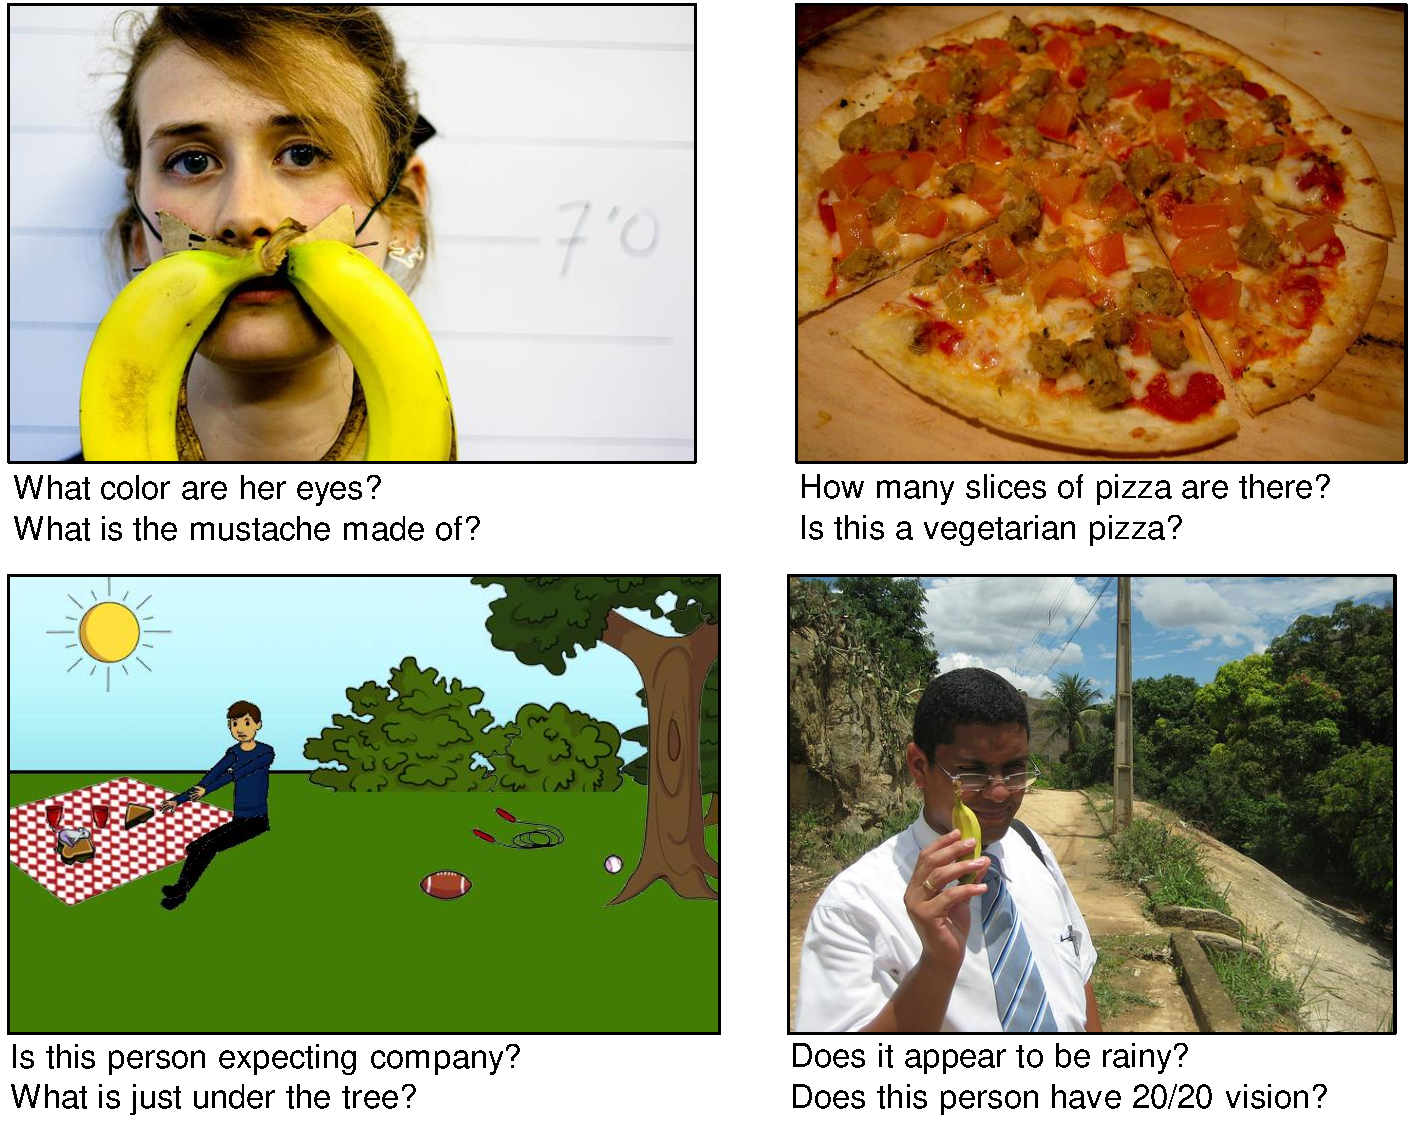
\includegraphics[width=1\linewidth]{figures/teaser_v2.pdf}
\caption{Examples of free-form, open-ended questions collected for images via Amazon Mechanical Turk.
Note that commonsense knowledge is needed along with a visual understanding of the scene
to answer many questions.}
\label{fig:teaser}
%\vspace{\captionReduceBot}
\end{figure}
%%%%%%%%%%%%%%%%%%%%%%%%%%%%%%%%%%%%%%%%%%%%%%%%%%%%%%%%%%%


%VQA meets both the desiderata defined above. \\
Open-ended questions require a potentially vast
set of AI capabilities to answer --
% DB: I think we should defend against these in the related work section. Right now, I think it
% flows better to "own" VQA.
%Unlike previous visual question and answer datasets that restrict
%their questions to specific types \cite{geman,fritz,BergECCV2010}. Some of the AI abilities required
%to answer our questions include
fine-grained recognition (\eg, ``What kind of cheese is on the pizza?''),
object detection (\eg, ``How many bikes are there?''),
activity recognition (\eg, ``Is this man crying?''),
knowledge base reasoning (\eg, ``Is this a vegetarian pizza?''),
and commonsense reasoning (\eg, ``Does this person have 20/20 vision?", ``Is this person expecting company?'').
%(\eg, ``Does this look like a pleasant place to relax?" or ``Is this a one-way street?''). 
%\dhruv{Need to incorporate vizwiz in intro.}
%As shown by \cite{vizwiz}, for applications such
%as helping the visually impaired, the diversity of visual questions is remarkable. Interestingly,
%these questions require detailed and specific information about the image for which generic
%image captions are of little use \cite{vizwiz}. Open-ended questions require a potentially vast
%set of AI capabilities to answer, unlike previous visual question and answer datasets that restrict
%their questions to specific types \cite{geman,fritz,BergECCV2010}. Some of the AI abilities required
%to answer our questions include
%fine-grained recognition (\eg, ``What type of pizza is this called?''),
%object detection (\eg, ``How many Post-it notes are on the table?''),
%activity recognition (\eg, ``What are these people doing?''),
%knowledge base reasoning (\eg, ``Is this a vegetarian pizza?''),
%and commonsense reasoning (\eg, ``Does this person have 20/20 vision?" or ``Is this person expecting company?'').
%%(\eg, ``Does this look like a pleasant place to relax?" or ``Is this a one-way street?''). 
VQA~\cite{geman,fritz,SongChun_video_queries,vizwiz} is also amenable to automatic quantitative evaluation, making it possible to effectively track progress on this task.
While the answer to many questions is simply ``yes'' or ``no'', the process for determining a correct answer is typically far from trivial (e.g.~in \figref{fig:teaser}, ``Does this person have 20/20 vision?'').
%While the process for determining a correct answer is typically far from trivial, the answer to many questions is simply ``yes'' or ``no'' (for instance in \figref{fig:teaser}, ``Does this person have 20/20 vision?''). 
 Moreover, since questions about images often tend to seek specific information, simple one-to-three word answers are sufficient for many questions. In such scenarios, we can easily evaluate a proposed algorithm by the number of questions it answers correctly.
In this paper, we present both an open-ended answering task and a multiple-choice
task \cite{richardson2013mctest,FITB_VP}. Unlike the open-ended task that requires a
free-form response, the multiple-choice task only requires an algorithm to pick from a predefined
list of possible answers.  
%We anticipate that the multiple-choice task will provide a reasonable
%{\it first step} towards VQA, while the open-ended task will become %more approachable (and can become more complex) as systems improve.

%VQA is its amenable to automatic quantitative evaluation. For many questions,
%simple one to three word answers are sufficient. While the process for determining a correct
%answer is typically far from trivial, the answer to many questions is simply ``yes'' or ``no''
%(for instance in \verify{Fig.~\ref{fig:teaser}}, ``Does this person have 20/20 vision?'').
%In this paper we present both an open-ended answering task and a multiple-choice
%task \cite{richardson2013mctest,FITB_VP}. Unlike the open-ended task that requires a
%free-form response, the multiple-choice task only requires an algorithm to pick from a predefined
%list of possible answers.

We present a large dataset that contains 204,721 images from the MS COCO
dataset \cite{coco} and a newly created abstract scene dataset \cite{ZitnickCVPR2013,Antol2014}
that contains 50,000 scenes. The MS COCO dataset has images depicting diverse and complex scenes that are effective at eliciting compelling and diverse questions. We collected a new dataset of ``realistic'' abstract scenes to enable research focused only on the high-level reasoning required for VQA by removing the need to parse real images. Three questions were collected for each image or scene. Each question was answered by ten subjects along with their confidence. The dataset contains over 760K questions with around 10M answers.
%\footnote{As of this submission,
%the dataset currently has 120,520 questions with 270,210 answers for 50,000 MS COCO
%images and 30,000 questions with 79,740 answers for 10,000 abstract scenes.}

%\textbf{Analysis.}
While the use of open-ended questions offers many benefits, it is still useful to understand the types of questions that are being asked and which types various algorithms may be
good at answering. To this end, we analyze the types of questions asked and the types of answers provided.
Through several visualizations, we demonstrate the astonishing diversity of the questions asked. We also explore how the information content of questions and their answers differs from image captions.
For baselines, we offer several approaches that use a combination of both text and state-of-the-art
visual features~\cite{AlexNet}. As part of the VQA initiative, we will organize an annual challenge and
associated workshop to discuss state-of-the-art methods and best practices.

VQA poses a rich set of challenges, many of which have been viewed as the holy grail of
automatic image understanding and AI in general. However, it includes as building blocks
several components that the CV, NLP, and KR \cite{NEEL,NEIL,Cyc,ConceptNet,Freebase} communities have made
significant progress on during the past few decades. VQA provides an attractive balance
between pushing the state of the art, while being accessible enough for the communities
to start making progress on the task.

%\larry{If we have space explicitly list contributions.}